%DO NOT MESS AROUND WITH THE CODE ON THIS PAGE UNLESS YOU %REALLY KNOW WHAT YOU ARE DOING
\chapter*{Experimental Research}
\addcontentsline{toc}{chapter}{Experimental Research}


\section{ Signal to Noise Ratio } \label{ Signal to Noise Ratio } 
\noindent  The MATLAB program for determining the signal to noise ratio was developed. The following parameter values were considered.

\begin{minipage}[b]{.40\textwidth}
   \centering
   \begin{tabular}{ | l | l |}
     \hline
     \textit{z / r} & uptp 50 m / 600 m \\ \hline
     \textit{bt} & mud, sand and gravel \\ \hline
     \textit{$v_{W}$} & 5, 15 and 25 knots \\ \hline
     \textit{S} & 33 ppt \\ \hline
     \textit{T} & $15^{\circ}$ \\ \hline
     \textit{c} & 1480 m/s \\ \hline
     \textit{SL} & 220 dB \\ \hline
     \textit{f} & 100 kHz \\ \hline
      $ \uptau $& $100 \mu s $\\ \hline
      \textit{DI} & 30 dB \\
     \hline
   \end{tabular}
  \end{minipage}\qquad
\begin{minipage}[b]{.40\textwidth}
   \centering
   \begin{tabular}{ | l | l |}
     \hline
      \textit{B} & 10 kHz \\ \hline
     \textit{$BP_{T}$} & 0 dB $(\pm 90^{\circ})$ \\ \hline
     \textit{$BP_{R}$} & 0 dB $(\pm 90^{\circ})$\\ \hline
     $2\theta_{\textit{h,R}} $ & $0.5^{\circ}$\\ \hline
     $2\theta_{\textit{h,T}} $ & $90^{\circ}$ \\ \hline
     $2\theta_{\textit{v,R}} $ & $180^{\circ}$ \\ \hline
     $2\theta_{\textit{v,T}} $ & $180^{\circ}$ \\ \hline
     \textit{$r_{S}$} & 0 m \\ \hline
      \textit{$z_{S}$} & 5 m \\ \hline
       \textit{TS} & $ -15 dB$ \\
   \hline
   \end{tabular}
   \end{minipage}
   \newpage
   
\noindent Signal to noise ratio (SNR) is a measure of how strong the signal of interest is with respect to the noise environment. The higher the SNR, the better the detection. The Figure 1, Figure 2 and Figure 3 show SNR as a function of depth and range for this particular sonar/environment scenario. In the images, colour is mapped to SNR where red is high and blue is low.



\noindent The Figure 1 shows the impact of wind speed on signal to noise ratio in the range of $\textit{r} (50, 600).$ The figure has been plotted for fixed value of wind speeds (5 kn, 15 kn and 25 kn) and the bottom type is considered to be mud. We can see from the Figure 1 that as the wind speed is increased from 5 kn to 25 kn, the signal to noise ratio decreases.

\begin{figure}[h]
\centering
\subfloat[first]{
  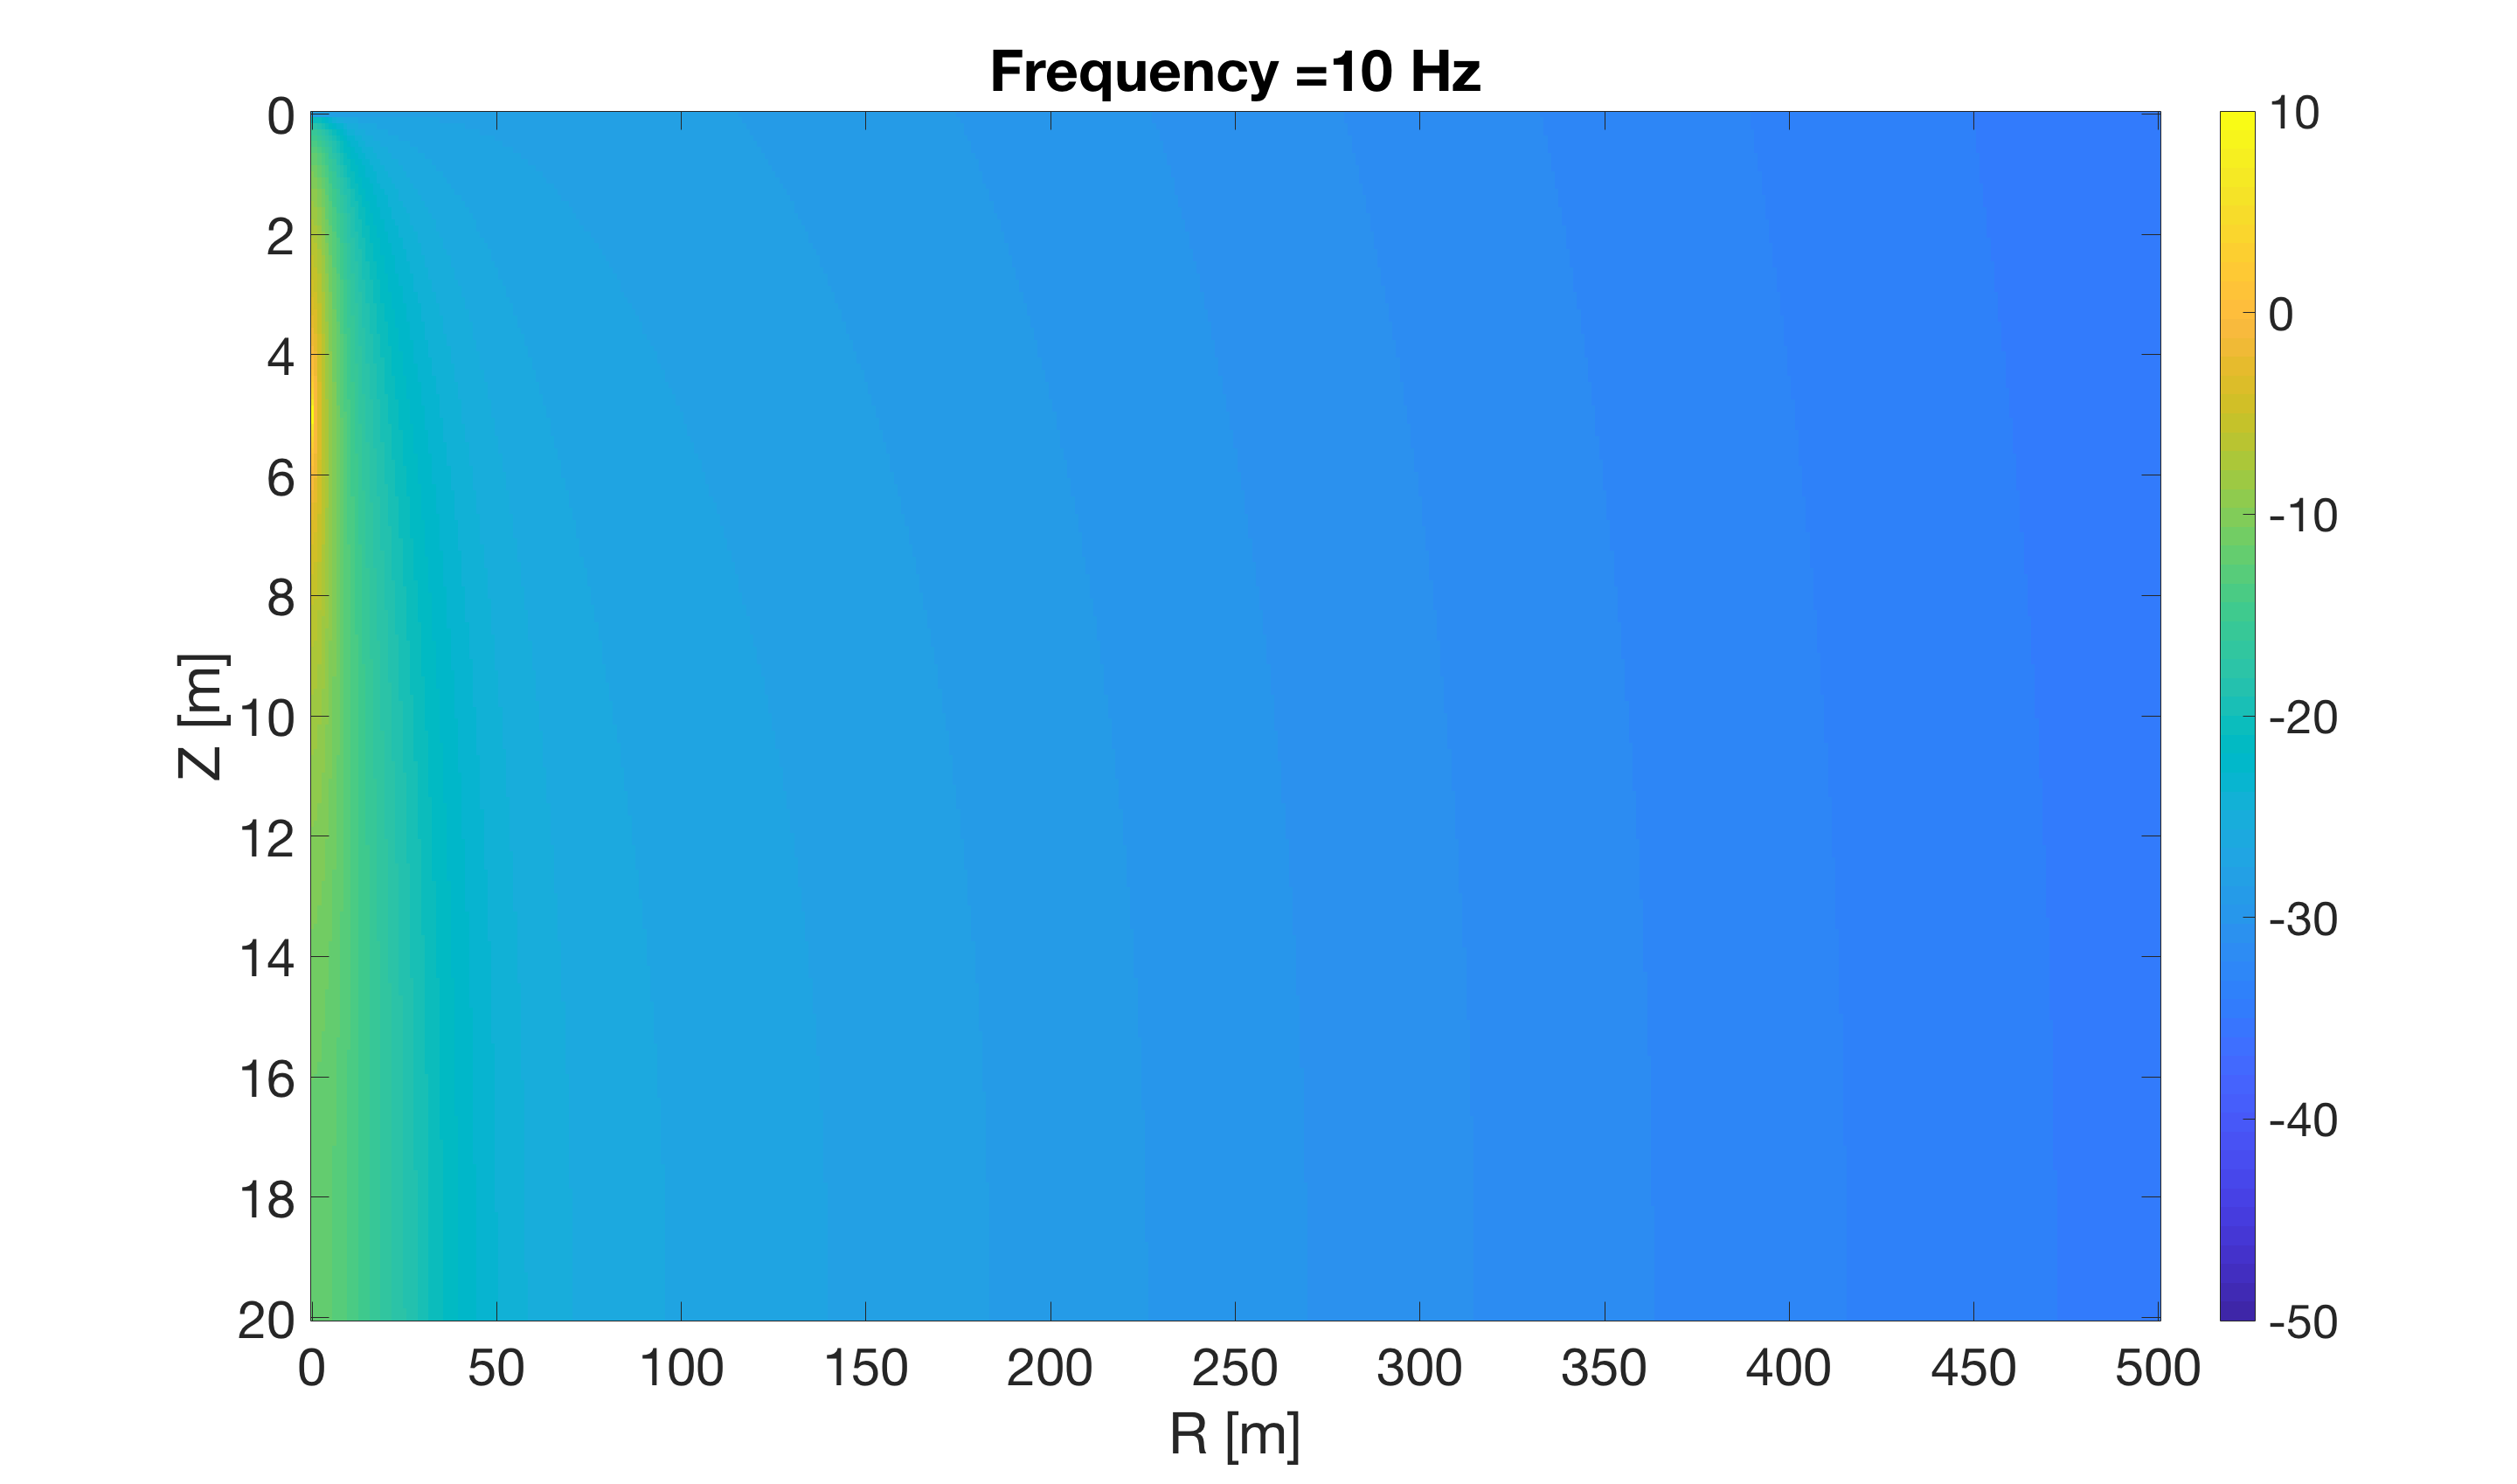
\includegraphics[width=95mm]{usp6_1.png}
}
\subfloat[second]{
  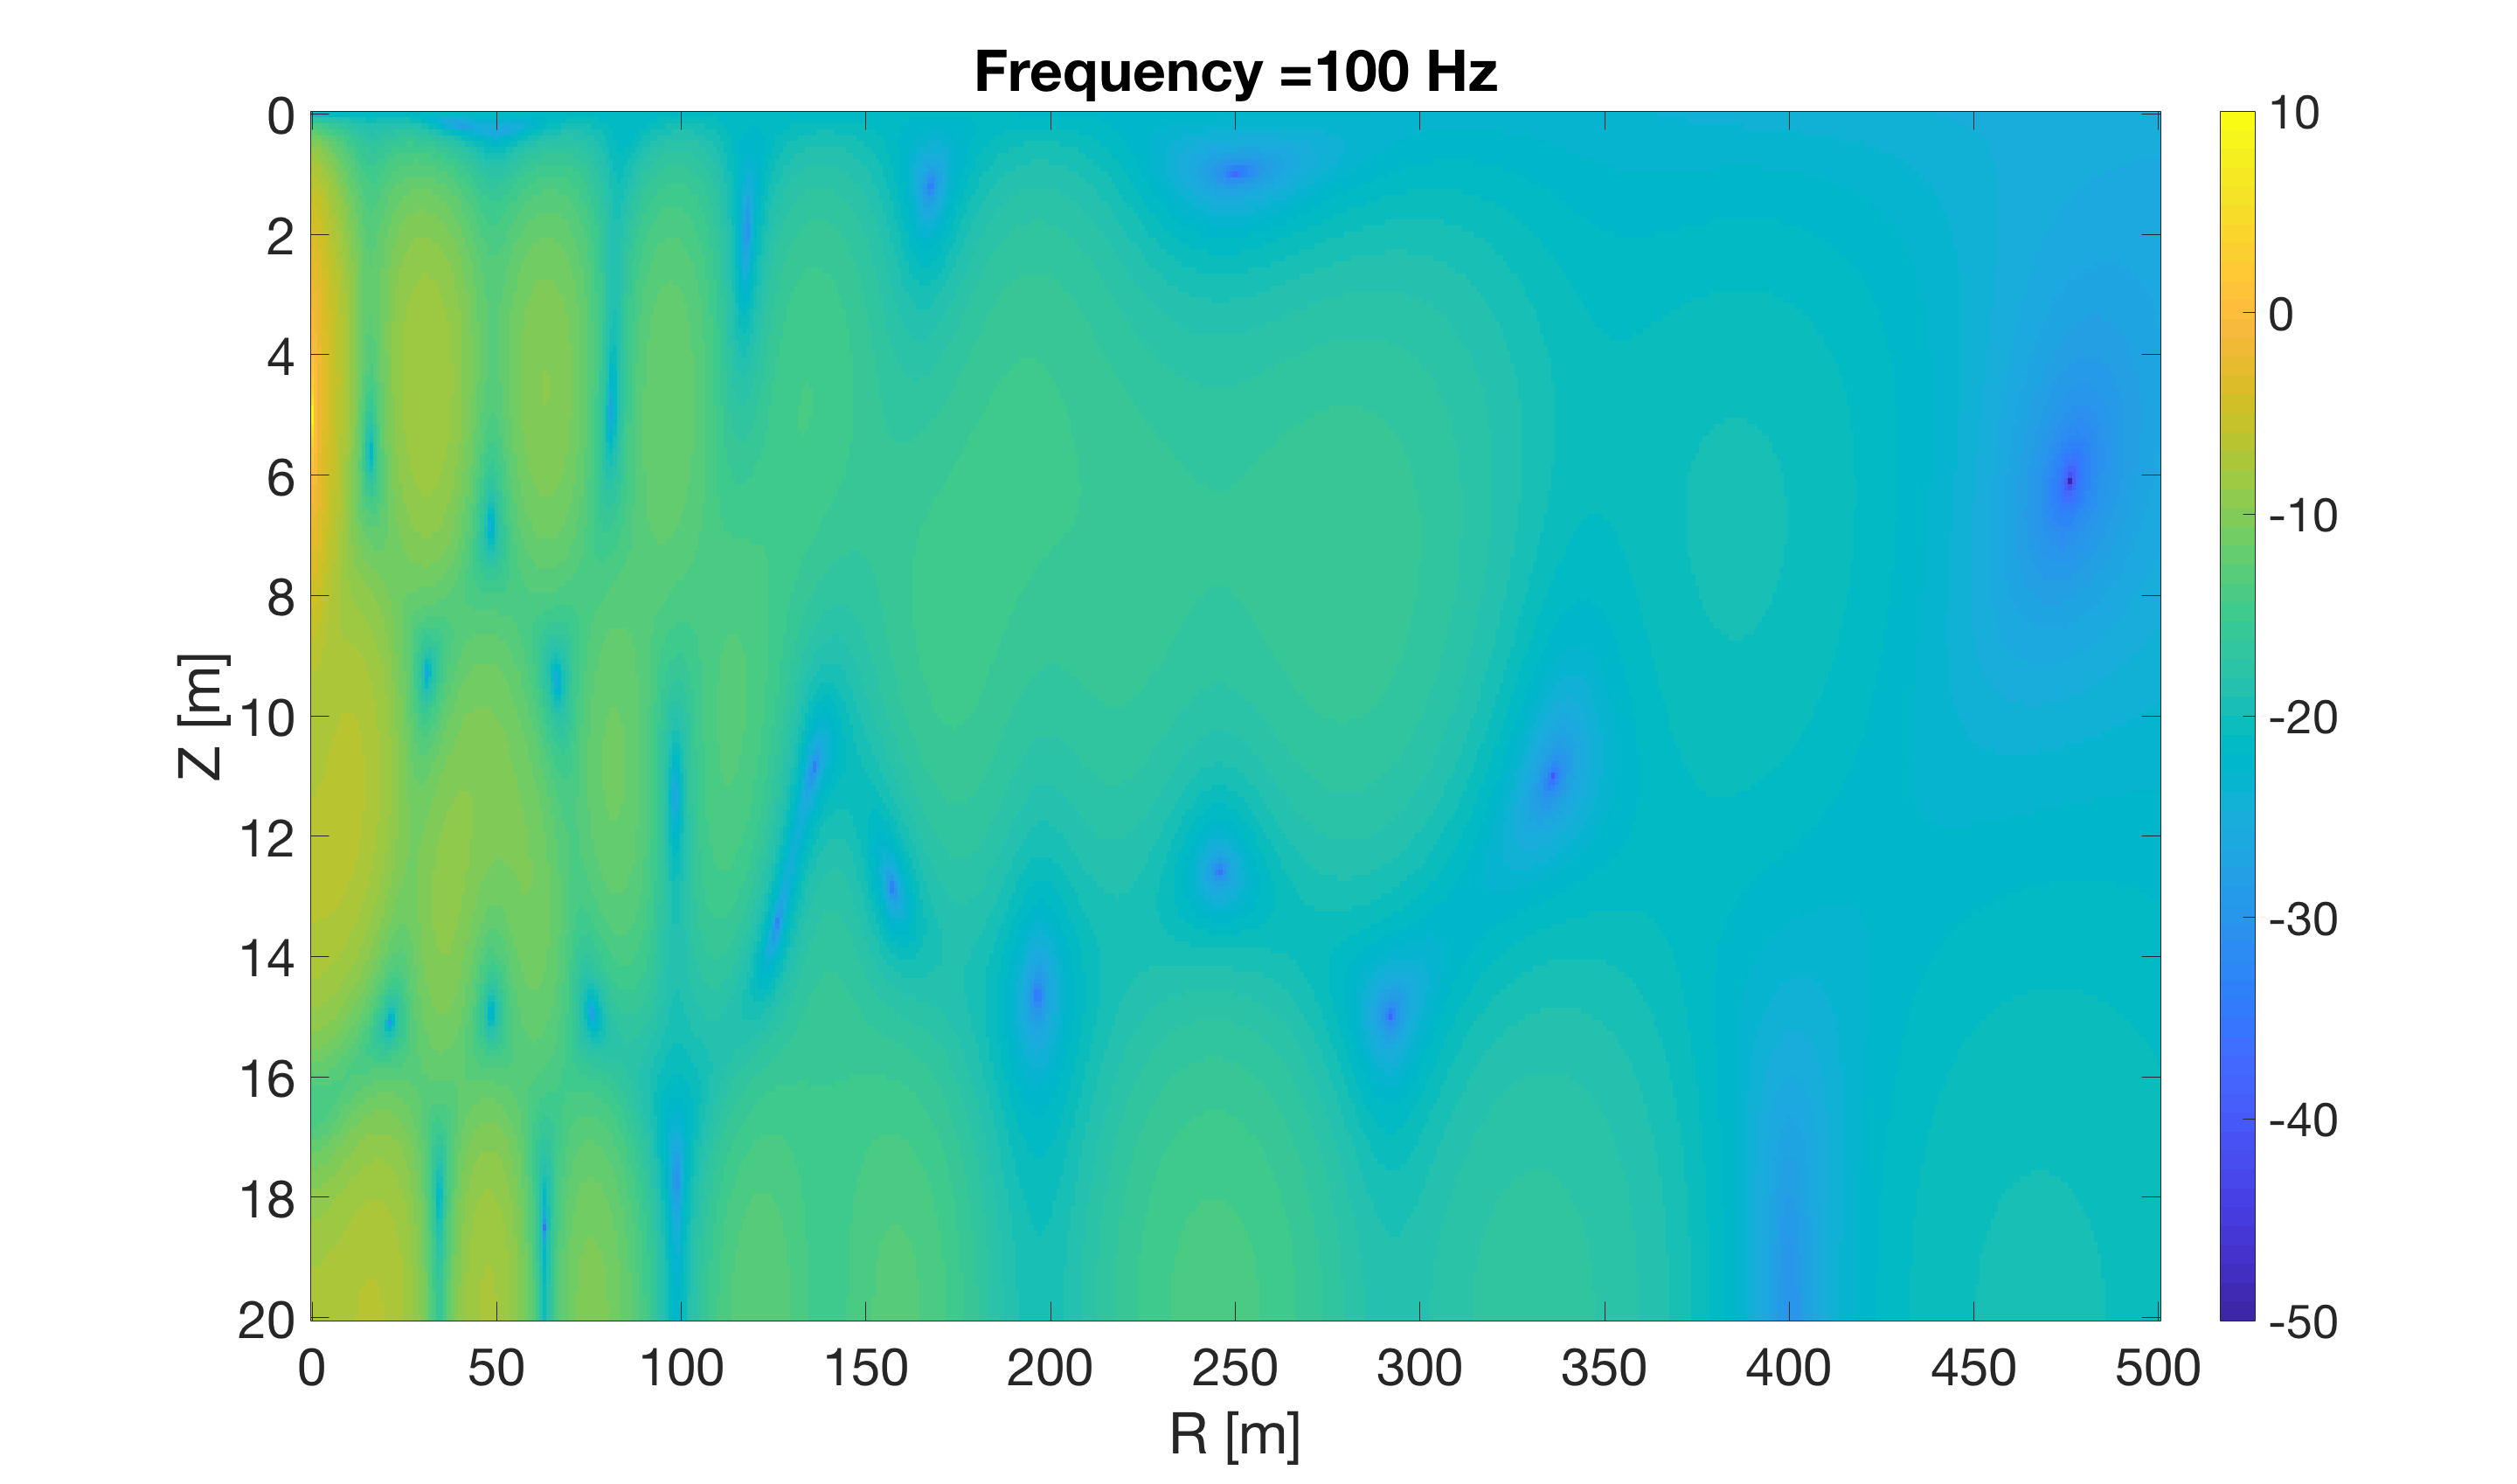
\includegraphics[width=95mm]{usp6_2.png}
}
\newline
\subfloat[third]{
  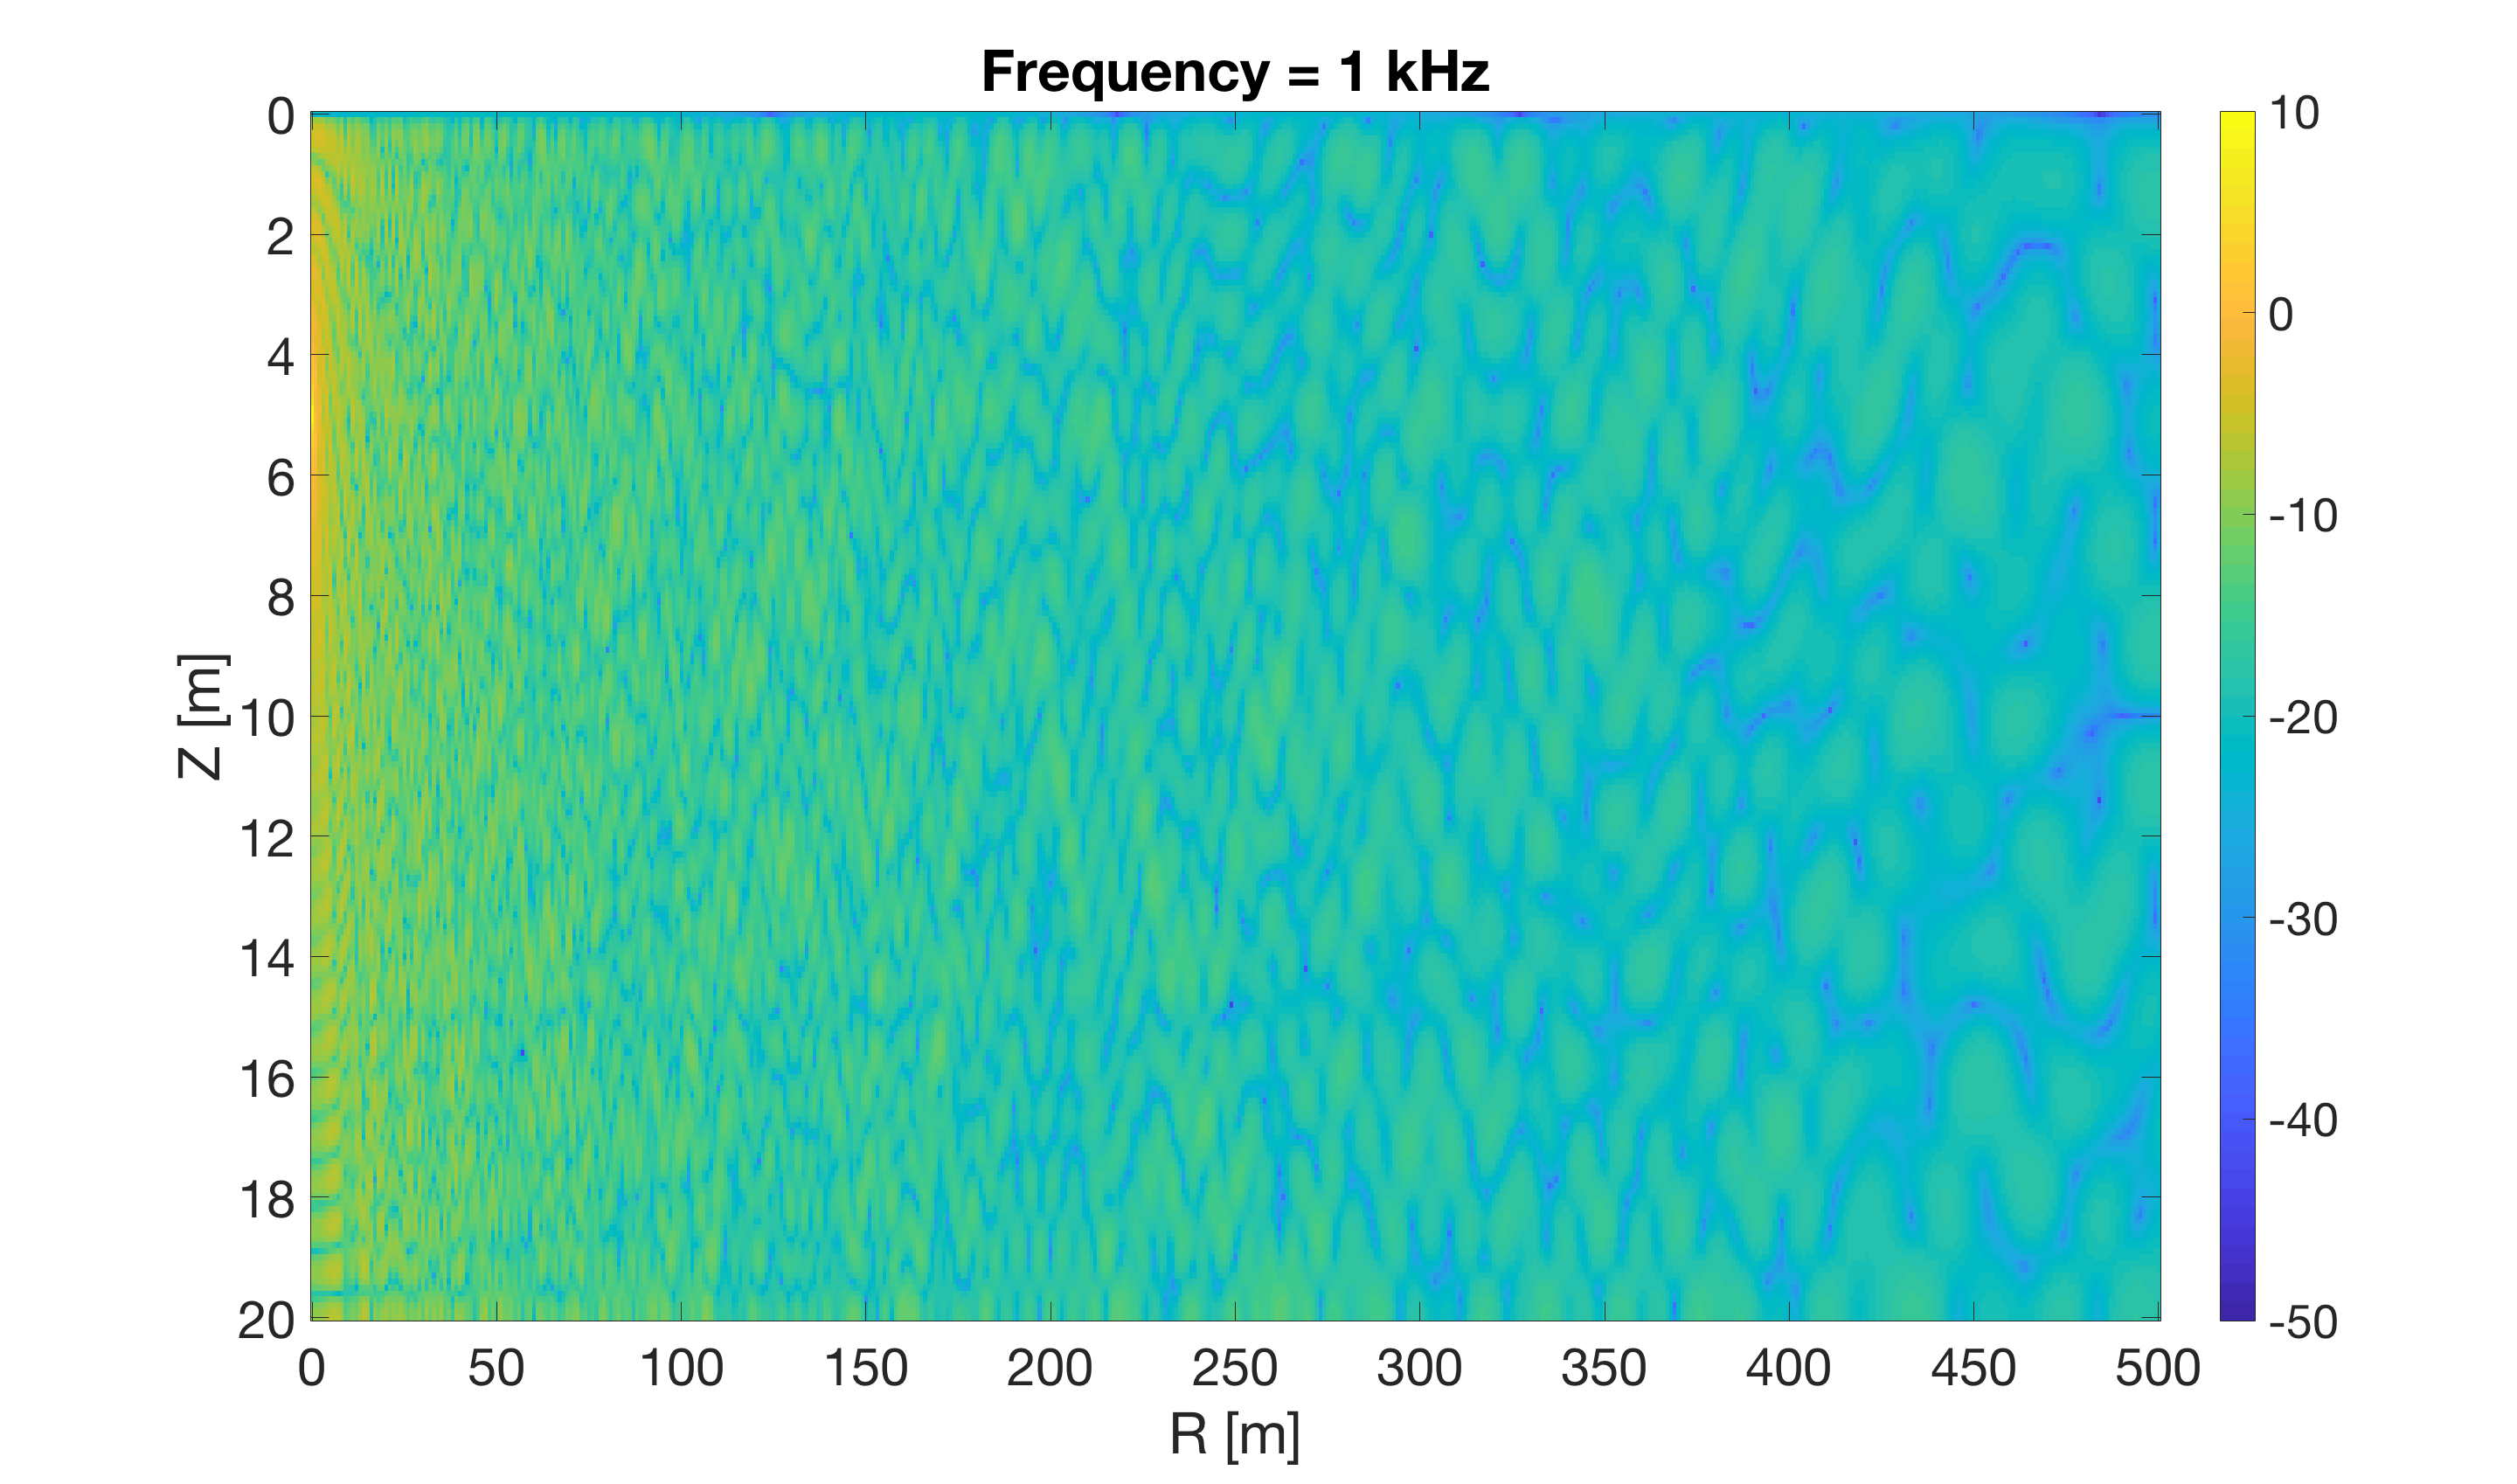
\includegraphics[width=95mm]{usp6_3.png}
}
\subfloat[forth]{
  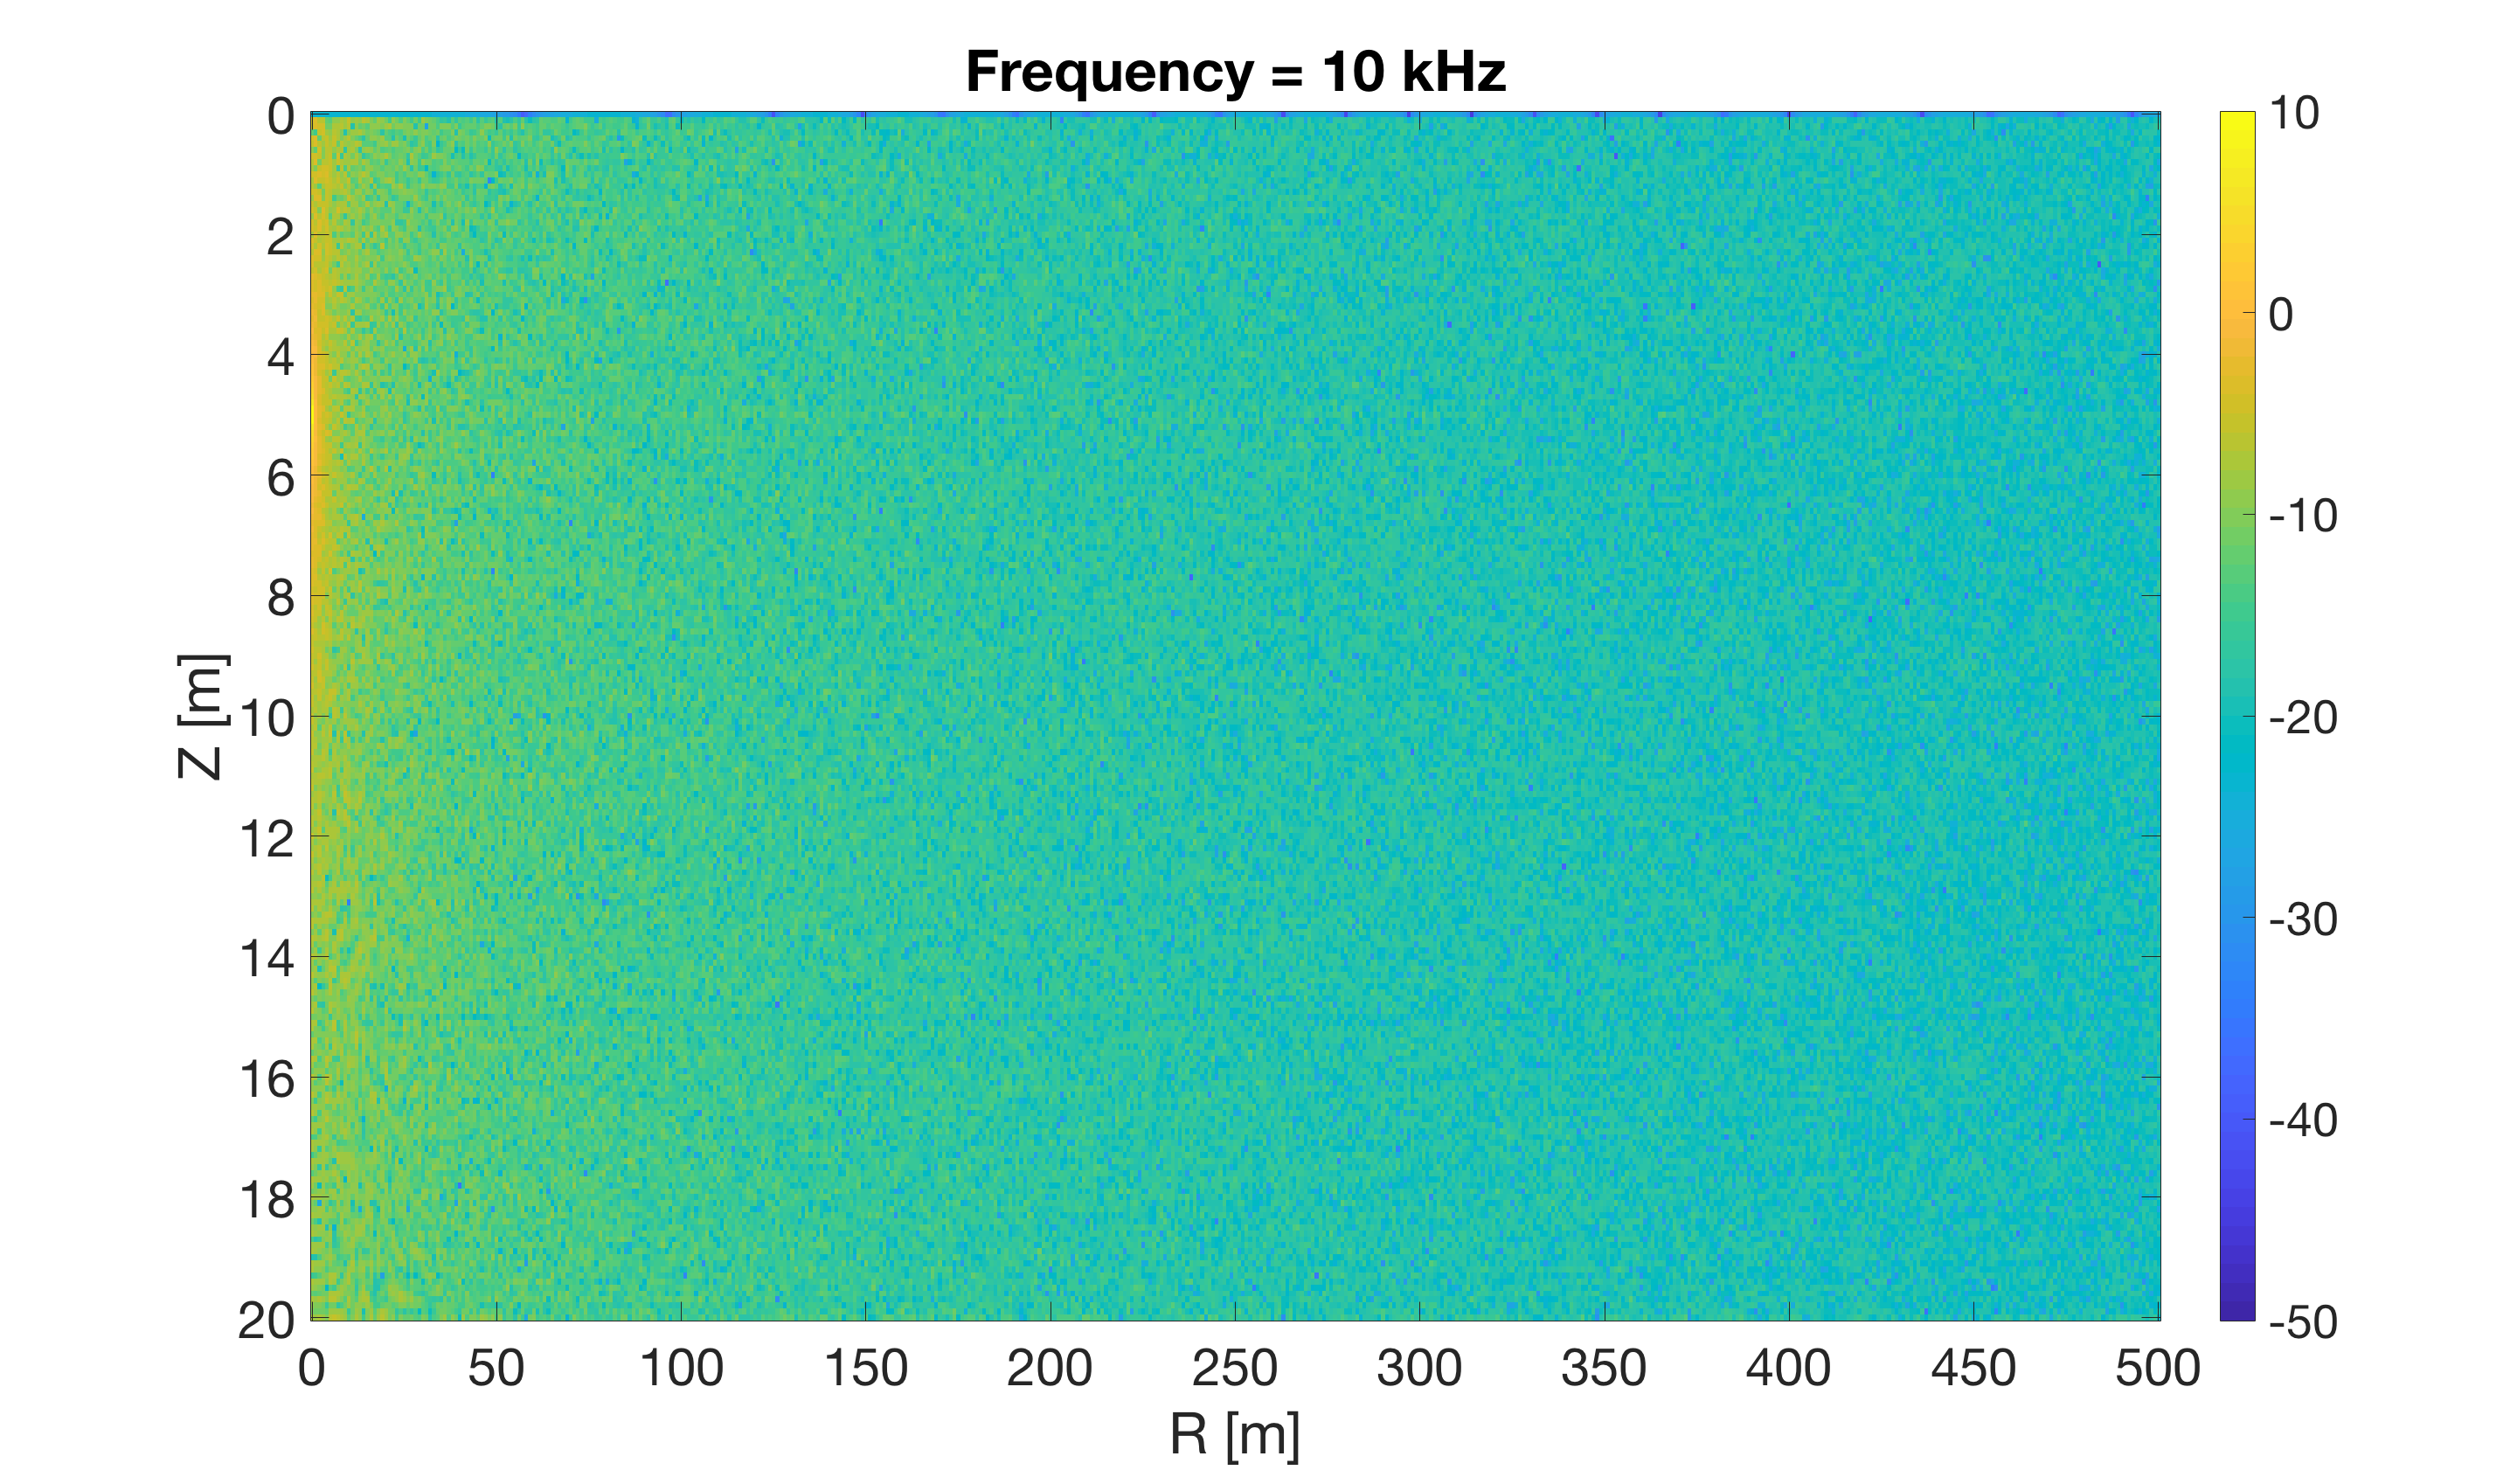
\includegraphics[width=95mm]{usp6_4.png}
}
\newline
\hbox to 18.5mm{}% !!
\subfloat[fifth]{
  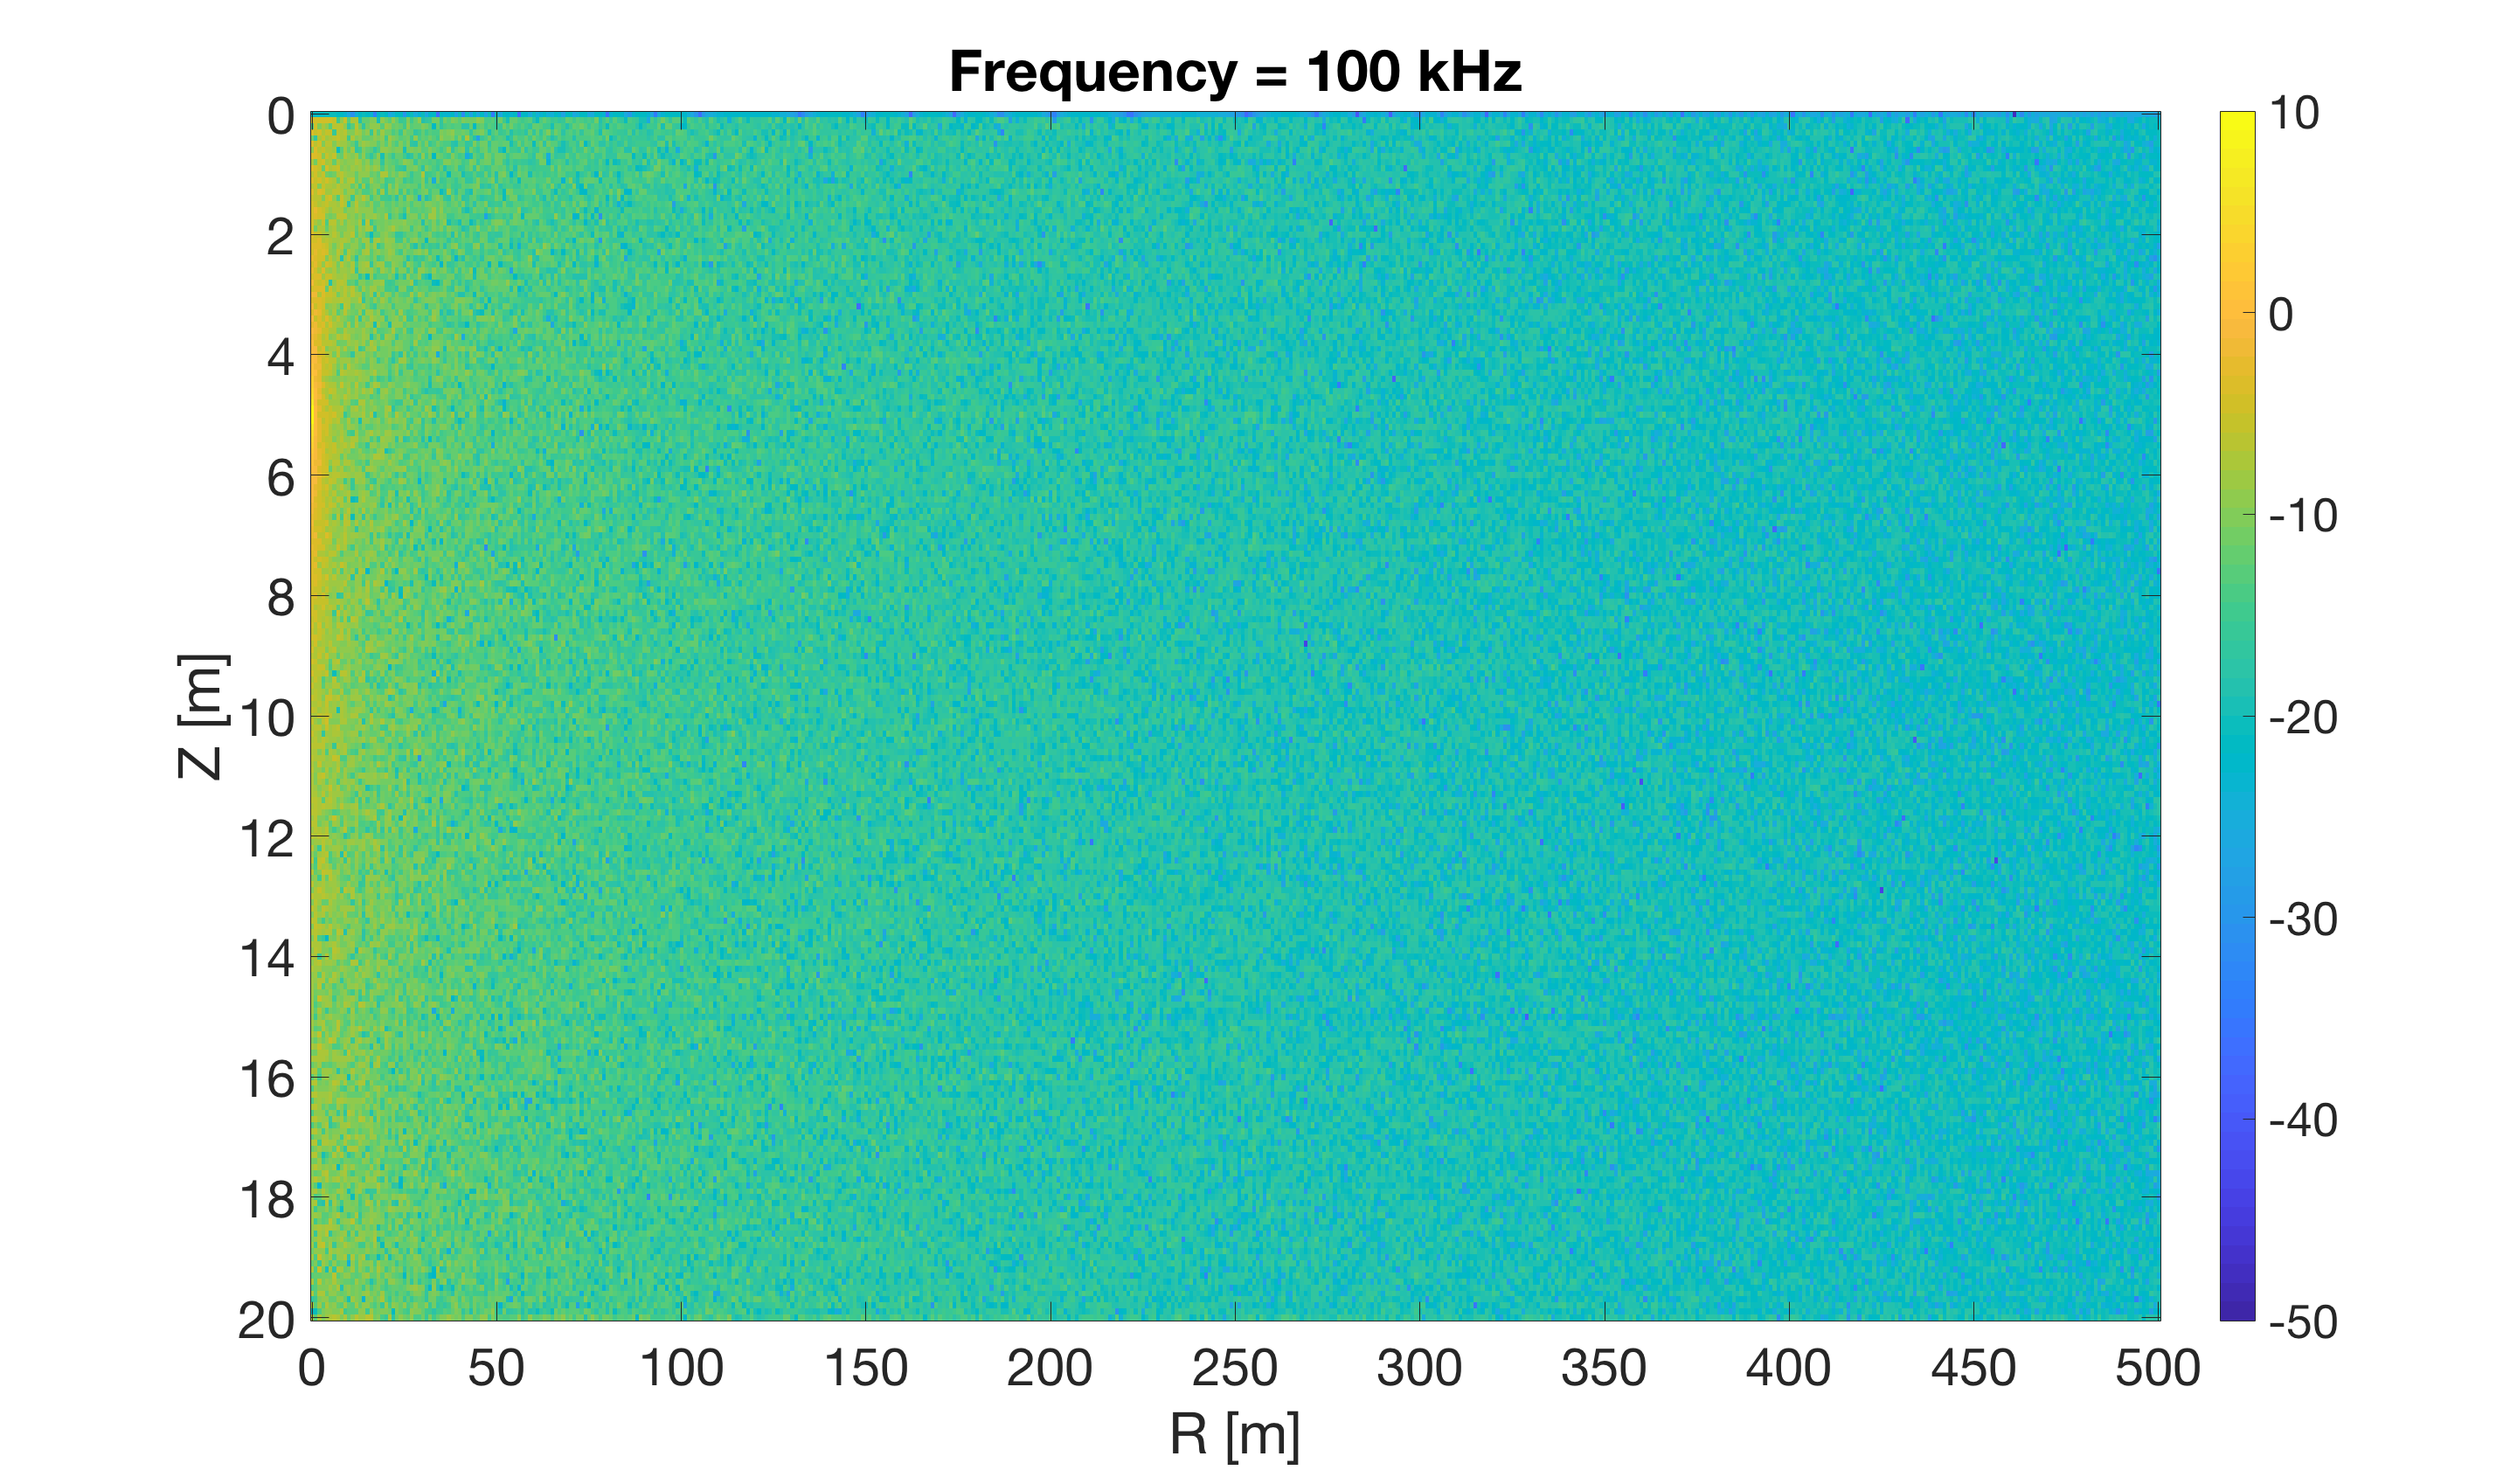
\includegraphics[width=90mm]{usp6_5.png}
}
\caption{Impact of sand as the bottom type and wind speed of 5, 15 and 25 knots on the signal to noise ratio}
\end{figure}




